\section{Семинар \thesection}
\subsection{Теория рассеяния. Борновское приближение}

В прошлом семинаре мы рассматривали метод парциальных волн для решения задачи рассеяния. Этот метод хорошо работает в случае сферической симметрии рассеивающего потенциала. Сейчас мы рассмотрим борновское приближение, в рамках которого мы считаем, что взаимодействие между рассеивающимися частицами является слабым, то есть волновая функция слабо отличается от плоской волны. По сути, метод Борна является применением теории возмущений для задачи квантового рассеяния. Для описания такого взаимодействия нам понадобится ввести функции Грина (также называемые пропагаторами) и определить интегральный вид уравнения Шрёдингера.

\subsubsection{Интегральное уравнение Шрёдингера. Функция Грина}

Начнем с рассмотрения стационарного уравнения Шрёдингера:
\[
-\frac{\hbar^2}{2m}\nabla^2\psi+V\psi=E\psi.
\]
Оно может быть записано как уравнение Гельмгольца, если мы положим $k=\sqrt{2mE}/\hbar$ и $Q=2mV\psi/\hbar^2$:
\[
(\nabla^2+k^2)\psi = Q.
\]

Предположим, что мы знаем решение уравнения Гельмгольца, у которого в правой части находится дельта-функция:
\[
(\nabla^2+k^2)G(\textbf{r})=\delta^3(\textbf{r}).
\]
$G(\textbf{r})$ -- это \textit{функция Грина} для уравнения Гельмгольца. Используя её и учитывая свойства дельта-функции, мы можем найти решение исходного уравнения на $\psi$ с помощью следующего интеграла:
\[
\psi(\textbf{r})=\int G(\textbf{r}-\textbf{r}_0)Q(\textbf{r}_0)d^3 \textbf{r}_0
\]

Мы можем найти её с помощью преобразования Фурье, которое позволит нам перейти от дифференциального уравнения к алгебраическому. Пусть
\[
G(\textbf{r}) = \frac{1}{(2\pi)^{3/2}}\int e^{i\textbf{s}\cdot\textbf{r}}g(\textbf{s})d^3\textbf{s}.
\]
Тогда,
\[
(\nabla^2+k^2)G(\textbf{r}) = \frac{1}{(2\pi)^{3/2}}\int\left[(\nabla^2+k^2)e^{i\textbf{s}\cdot\textbf{r}}\right]g(\textbf{s})d^3\textbf{s}.
\]
Заметим, что
\[
\nabla^2e^{i\textbf{s}\cdot\textbf{r}}=- s^2 e^{i \textbf{s} \cdot \textbf{r}}, \quad \delta^3(\textbf{r})=\frac{1}{(2\pi)^3}\int e^{i\textbf{s}\cdot\textbf{r}}d^3\textbf{s}.
\]
Подставляя эти выражения в уравнение Гельмгольца, мы получим
\[
\frac{1}{(2\pi)^{3/2}}\int(-s^2+k^2)e^{i\textbf{s}\cdot\textbf{r}}g(\textbf{s})d^3\textbf{s}=\frac{1}{(2\pi)^3}\int e^{i\textbf{s}\cdot\textbf{r}}d^3\textbf{s}.
\]
Отсюда мы можем увидеть, что 
\[
g(\textbf{s})=\frac{1}{(2\pi)^{3/2}(k^2-s^2)} \implies G(\textbf{r})=\frac{1}{(2\pi)^3}\int e^{i\textbf{s}\cdot\textbf{r}}\frac{1}{k^2-s^2}d^3 \textbf{s}.
\]

Осталось всего ничего -- взять этот интеграл. Для удобства перейдем в сферическую систему координат $(s,\theta,\varphi)$, направив полярную ось по $\textbf{r}$. В таком случае $\textbf{s}\cdot \textbf{r} = sr\cos\theta$, а наш интеграл принимает вид
\[
G(\textbf{r})=\frac{1}{(2\pi)^3}\int\limits_0^{2\pi}d\varphi\int\limits_{0}^{+\infty}ds\int\limits_0^{\pi} e^{isr\cos\theta} \frac{1}{k^2-s^2} s^2\sin\theta d\theta
\]

Интеграл по $\varphi$ тривиален и равен $2\pi$, по $\theta$ тоже берется достаточно просто:
\[
\int\limits_0^{\pi} e^{isr\cos\theta}\sin\theta d\theta=-\left.\frac{e^{isr\cos\theta}}{isr}\right|_0^{\pi}=2\frac{\sin(sr)}{sr}
\]

Оставшийся интеграл не так прост:
\[
G(\textbf{r})=\frac{1}{(2\pi)^2}\frac{2}{r}\int\limits_0^{+\infty}\frac{s\sin(sr)}{k^2-s^2}ds=\frac{1}{4\pi^2 r}\int\limits_{-\infty}^{+\infty}\frac{s\sin(sr)}{k^2-s^2}ds.
\]
Перейдем от синуса к комплексным экспонентам и распишем знаменатель по формуле разности квадратов:
\[
G(\textbf{r})=\frac{i}{8\pi^2 r}\left[\int\limits_{-\infty}^{+\infty}\frac{se^{isr}}{(s-k)(s+k)}ds-\int\limits_{-\infty}^{+\infty}\frac{se^{-isr}}{(s-k)(s+k)}ds\right]=\frac{i}{8\pi^2 r}(I_1-I_2).
\]
Эти интегралы можно посчитать с помощью интегральной формулы Коши 
\[
\oint\frac{f(z)}{z-z_0}dz=2\pi i f(z_0),
\]
если $z_0$ лежит внутри контура интегрирования. Если не лежит, то интеграл равен нулю. В данном случае все интегрирование ведется вдоль действительной оси с обходом полюсов $\pm k$. Для удобства, мы выберем следующий способ обхода: над $-k$ и под $+k$ (рис. \ref{fig 4.1}).

\begin{figure}[ht]
\centering
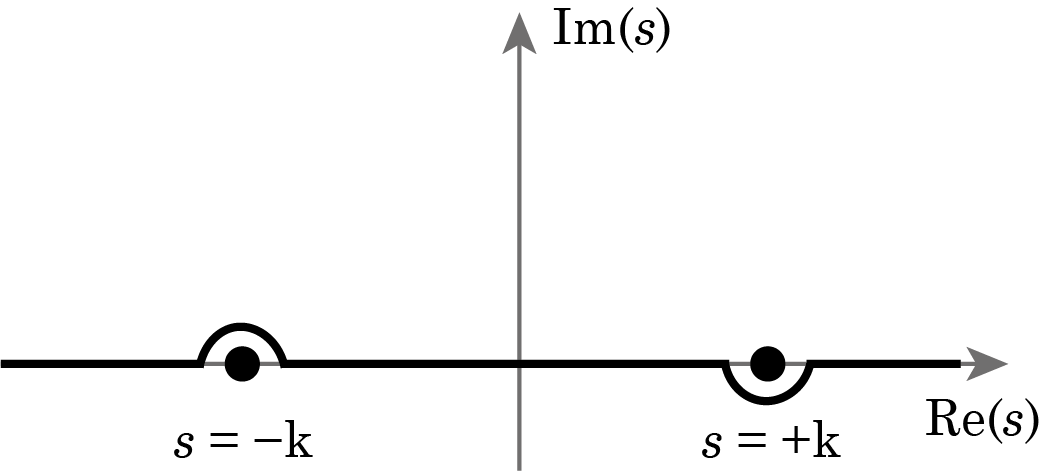
\includegraphics[scale=1]{class_5/images/poles-skirting.png}
\caption{Обход полюсов}
\label{fig 4.1}
\end{figure}

Для каждого из интегралов $I_1$ и $I_2$ мы должны замкнуть контур так, чтобы на бесконечности был нулевой вклад. В случае $I_1$, $e^{isr}$ занулится, если Im$(s)\to+\infty$, то есть контур следует замкнуть сверху (рис. \ref{fig 4.2 a}). Тогда, внутри контура останется один полюс $s=+k$, откуда
\[
I_1=\oint\left[\frac{se^{isr}}{s+k}\right]\frac{1}{s-k}ds=2\pi i\left.\left[\frac{se^{isr}}{s+k}\right]\right|_{s=k}=i\pi e^{ikr}.
\]

\begin{figure}[ht]
  \centering
  \subfloat[Замыкание контура сверху]{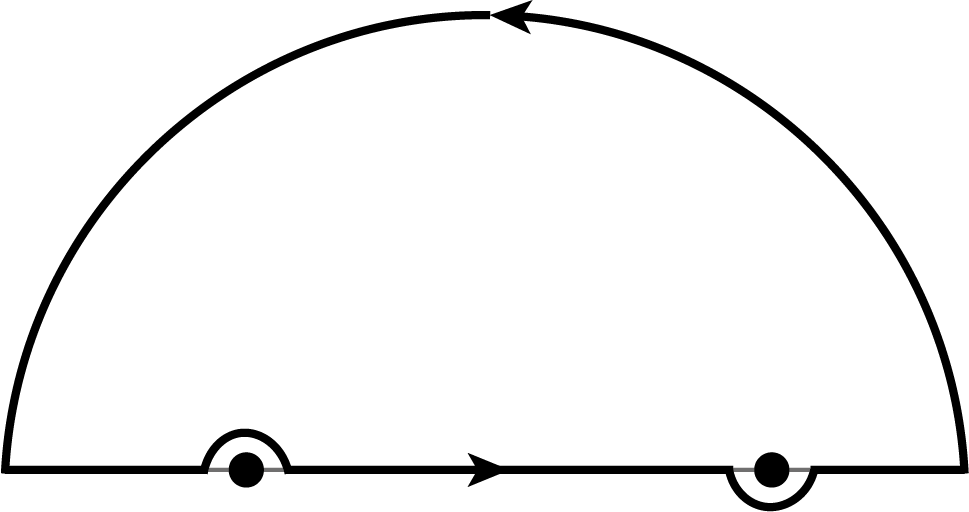
\includegraphics[scale=0.5]{class_5/images/contour a.png}\label{fig 4.2 a}}
  \hspace{5em}
  \subfloat[Замыкание контура снизу]{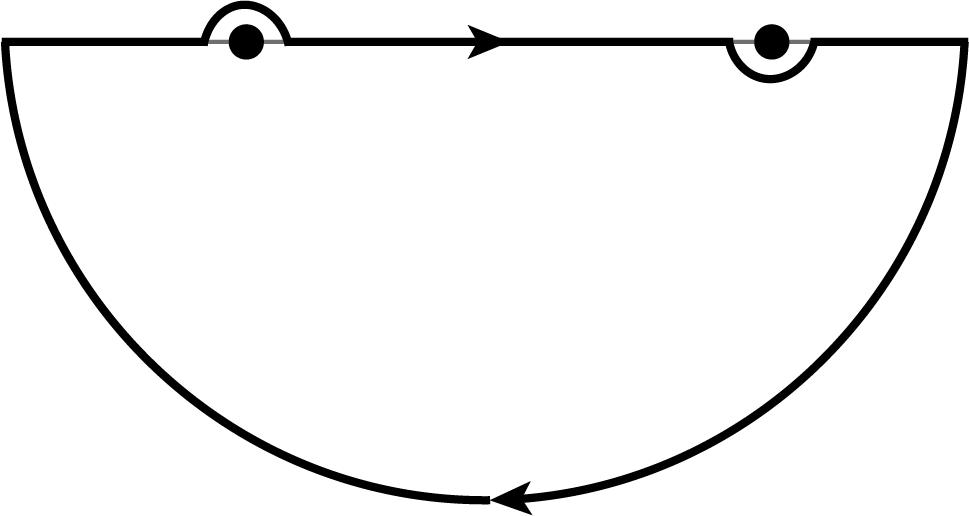
\includegraphics[scale=0.5]{class_5/images/contour b.png}\label{fig 4.2 b}}
  \caption{}
\end{figure}

Напротив, в случае $I_2$, множитель $e^{-isr}$ стремится к нулю при $Im(s)\to-\infty$, то есть контур замкнется снизу (рис. \ref{fig 4.2 b}). В таком случае контур оказывается ориентирован \textit{по} часовой стрелке, а не против, поэтому нам надо брать интеграл с отрицательным знаком:
\[
I_2=-\oint\left[\frac{se^{-isr}}{s-k}\right]\frac{1}{s+k}ds=-2\pi i\left.\left[\frac{se^{-isr}}{s-k}\right]\right|_{s=-k}=-i\pi e^{ikr}.
\]

Наконец, можем выписать функцию Грина
\[
G(\textbf{r})=\frac{i}{8\pi^2 r}\left[i\pi e^{ikr}-(-i\pi e^{ikr})\right]=-\frac{e^{ikr}}{4\pi r}.
\]
Важно отметить, что эта функция Грина для уравнения Гельмгольца не является единственной. Например, мы могли бы выбрать другие пути обхода полюсов, и получили бы другой результат (который также был бы верным). В общем случае, мы можем добавить к $G(\textbf{r})$ любую функцию $G_0(\textbf{r})$, которая удовлетворяет однородному уравнению Гельмгольца:
\[
(\nabla^2+k^2)G_0(\textbf{r})=0.
\]

Кроме того, обсудим, что такое пропагаторы, и как они связаны с функцией Грина. Как мы уже сказали, функция Грина -- это \textit{любое} решение уравнения
\[
LG(x-y)=\delta(x-y)
\]
для заданного дифференциального оператора $L = L(x)$. В свою очередь, пропагатор -- это конкретно выбранная (с помощью начальных или граничных условий) функция Грина. Физически пропагатор определяет амплитуду вероятности перемещения частицы из одной точки пространства (пространства-времени) в другое. В данном случае мы выбрали конкретный обход полюсов, что позволило нам зафиксировать выражение для функции Грина. В квантовой теории поля, например, решается \textit{нестационарное} уравнение Шрёдингера, и различные обходы полюсов позволяют получать различные пропагаторы: опережающий, запаздывающий и пропагатор Фейнмана. Первый описывает распространение процессов ``из будущего в прошлое'', второй -- ``из прошлого в будущее'', а третий описывает процессы ``из прошлого в будущее'' для обычных частиц и наоборот для античастиц.

Теперь мы можем вернуться к выражению для волновой функции. Подставив в неё найденную функцию Грина, получим:
\[
\psi(\textbf{r})=\psi_0(\textbf{r})-\frac{m}{2\pi\hbar^2}\int\frac{e^{ik|\textbf{r}-\textbf{r}_0|}}{|\textbf{r}-\textbf{r}_0|}V(\textbf{r}_0)\psi(\textbf{r}_0)d^3\textbf{r}_0,
\]
где $\psi_0$ удовлетворяет уравнению Шрёдингера для свободной частицы $(\nabla^2+k^2)\psi_0=0$.

Выписанная выше формула называется интегральной формой уравнения Шрёдингера. Мы уже встречались с похожей формулой в первом семестре, когда переходили от координатного к импульсной форме УШ. Может показаться, что это -- решение уравнения, однако важно заметить, что в правой части под интегралом также присутствует $\psi$, то есть для того, чтобы найти волновую функцию, надо уже её знать. Тем не менее эта интегральная форма является полезной, и имеет важное применение в теории рассеяния. 

\subsubsection{Первое борновское приближение}

Поработаем с полученным выше интегральным уравнением Шрёдингера. Будем считать, что рассеивающий потенциал $V(\textbf{r}_0)$ локализован в окрестности $\textbf{r}_0=0$. Мы хотим вычислить $\psi(\textbf{r})$ в точке, сильно отдаленной от рассеивающего центра, т.е. при $|\textbf{r}|\gg|\textbf{r}_0|$. В таком случае
\[
|\textbf{r}-\textbf{r}_0|^2=r^2-2\textbf{r}\cdot\textbf{r}_0+r_0^2\approx r^2 - 2\textbf{r}\cdot\textbf{r}_0=r^2\left(1-2\frac{\textbf{r}\cdot\textbf{r}_0}{r^2}\right)
\]

Введем обозначение $\hat{\textbf{r}}=\textbf{r}/r$, и перепишем $|\textbf{r}-\textbf{r}_0|\approx r-\hat{\textbf{r}}\cdot\textbf{r}_0$. Кроме того, обозначим $\textbf{k}=k\hat{\textbf{r}}$. Тогда
\[
e^{ik|\textbf{r}-\textbf{r}_0|}\approx e^{ikr}e^{-i\textbf{k}\cdot\textbf{r}_0},
\]
и, следовательно,
\[
\frac{e^{ik|\textbf{r}-\textbf{r}_0|}}{|\textbf{r}-\textbf{r}_0|}\approx\frac{e^{ikr}}{r}e^{-\textbf{k}\cdot\textbf{r}_0}.
\]

В теории рассеяния мы считаем $\psi_0$ падающей плоской волной, то есть $\psi_0( \textbf{r} ) = A e^{ikz}$. Тогда, подставив все полученные приближения в интегральное уравнение Шрёдингера, получим:
\[
\psi(\mathbf{r})\approx Ae^{ikz}-\frac{m}{2\pi\hbar^2}\frac{e^{ikr}}{r}\int e^{-\mathbf{k}\cdot\mathbf{r}_0}V(\mathbf{r}_0)\psi(\mathbf{r}_0)d^3\mathbf{r}_0.
\]
Сравнивая это выражение с формулой из предыдущего семинара
\[
\psi(r,\,\theta)\approx A\left[e^{ikz} + f(\theta)\frac{e^{ikr}}{r}\right],
\]
можем сразу выписать амплитуду рассеяния:
\[
f(\theta, \, \varphi)=-\frac{m}{2\pi\hbar^2 A}\int e^{-\textbf{k}\cdot \textbf{r}_0}V(\textbf{r}_0)\psi(\textbf{r}_0)d^3\textbf{r}_0.
\]

До этого момента мы пользовались лишь тем фактом, что $r$ -- большое. Теперь добавим к этому еще и приближение Борна. Предположим, что падающая волна практически не изменяется от взаимодействия с потенциалом, то есть снова вернемся к теории возмущения, считая рассеивающий потенциал малым возмущением. Тогда,
\[
\psi(\textbf{r}_0)\approx\psi_0(\textbf{r}_0)=Ae^{ikz_0}=Ae^{i\textbf{k}'\cdot\textbf{r}_0},
\]
где
\[
\textbf{k}'=k\hat{z}.
\]
Иначе говоря, векторы $\textbf{k}'$ и $\textbf{k}$ равны по модулю, но отличаются по направлению: $\textbf{k}'$ сонаправлен с падающей волной, в то время как $\textbf{k}$ указывает на направление волны после рассеяния. Величина $\hbar(\textbf{k}-\textbf{k}')$ отвечает за изменение импульса при рассеянии.

Выходит, что в приближении Борна амплитуда рассеивания равна
\[
f(\theta,\,\varphi)\approx-\frac{m}{2\pi\hbar^2}\int e^{i(\textbf{k}'-\textbf{k})\cdot\textbf{r}_0}V(\textbf{r}_0)d^3\textbf{r}_0.
\]
В частности, если рассматривать рассеяние при низких энергиях (длинноволновое), то экспоненциальный множитель в интеграле примерно постоянен ($e^{i(\textbf{k}'-\textbf{k})\cdot\textbf{r}_0}\approx 1$), что позволяет упростить амплитуду рассеяния:
\[
f(\theta, \, \varphi)=-\frac{m}{2\pi\hbar^2}\int V(\textbf{r})d^3\textbf{r}.
\]

Для примера сразу рассмотрим неупругое рассеяние при низких энергиях (отметим, что жесткое рассеяние с помощью приближения Борна рассмотреть не получится, так как при $V_0=\infty$ интеграл расходится). 

\exercise
Пусть 
\[
V(\textbf{r})=\begin{cases}
    V_0, &r\leq a, \\ 0, &r>a.
\end{cases}
\]
В случае низкой энергии, амплитуда рассеяния будет равна
\[
f(\theta, \, \varphi)\approx-\frac{m}{2\pi\hbar^2}V_0\left(\frac{4}{3}\pi a^3\right),
\]
а дифференциальное сечение рассеяния:
\[
\frac{d\sigma}{d\Omega}=|f|^2\approx\left(\frac{2mV_0 a^3}{3\hbar^2}\right)^2.
\]
Полное сечение рассеяния в таком случае равно
\[
\sigma\approx4\pi\left(\frac{2mV_0 a^3}{3\hbar^2}\right)^2.
\]
\csquare{darklavender}

В наиболее интересном для нас случае сферически-симметричного потенциала ($V(\textbf{r})=V(r)$) приближение Борна можно дополнительно упростить. Определим $\boldsymbol{\kappa}=\textbf{k}'-\textbf{k}$ и направим полярную ось в сферической системе координат вдоль этого вектора $\boldsymbol{\kappa}$. Тогда,
\[
(\textbf{k}'-\textbf{k})\cdot\textbf{r}_0=\kappa r_0\cos\theta_0,
\]
а амплитуда рассеяния будет иметь следующий вид:
\[
f(\theta)\approx-\frac{m}{2\pi\hbar^2}\iiint e^{i\kappa r_0\cos\theta_0}\,V(r_0)\,r_0^2\sin\theta_0\,dr_0\,d\theta_0\,d\varphi_0.
\]
Вычисляя интегралы по $\theta_0$ и $\varphi_0$, получим
\[
f(\theta)\approx-\frac{2m}{\hbar^2\kappa}\int\limits_0^{+\infty}r\,V(r)\,\sin(\kappa r)\,dr.
\]
Заметим, что зависимость амплитуды от угла скрыта в $\kappa$, так как по теореме косинусов $\kappa = 2k\sin(\theta/2)$.

Важным примером сферически-симметричного потенциала является потенциал Юкавы\footnote{Юкава предложил этот потенциал для описания сильного (протон-нейтронного) взаимодействия. Он предполагал наличие мезонного обмена. Сейчас известно, что этот потенциал не описывает сильное взаимодействие в полной степени, но неплохо работает на расстояниях порядка 2 фм и энергии взаимодействия меньшей, чем 500 МэВ}, который играет большую роль при рассмотрении сильного взаимодействия. Этот потенциал выглядит следующим образом:
\[
V(r)=\beta\frac{e^{-\mu r}}{r},
\]

где $\beta, \; \mu$ -- константы. Тогда, пользуясь приближением Борна, выпишем
\[
f(\theta)\approx-\frac{2m\beta}{\hbar^2\kappa}\int\limits_0^{+\infty}e^{-\mu r}\,\sin(\kappa r)\,dr=-\frac{2m\beta}{\hbar^2(\mu^2+\kappa^2)}.
\]
Данный интеграл считается путем интегрирования по частям два раза.

Ещё один известный пример -- это рассеяние Резерфорда. Если в потенциале Юкавы положить $\beta=q_1 q_2/4\pi\epsilon_0, \; \mu=0$, то он превращается в потенциал Кулона, который используется для описания электрического взаимодействия двух точечных зарядов. В данном случае амплитуда рассеяния
\[
f(\theta)\approx-\frac{2mq_1 q_2}{4\pi\epsilon_0\hbar^2\kappa^2}= \frac{q_1 q_2}{16\pi\epsilon_0 E\sin^2(\theta/2)},\quad \kappa=2k\sin\frac{\theta}{2}, \; k=\frac{\sqrt{2mE}}{\hbar}.
\]

Дифференциальное сечение рассеяния же полностью совпадает с формулой Резерфорда:
\[
\frac{d\sigma}{d\Omega}=\left[\frac{q_1 q_2}{16\pi\epsilon_0 E\sin^2(\theta/2)}\right]^2.
\]

Получается, в случае потенциала Кулона и классика, и приближение Борна, и квантовая теория приводят к одному и тому же результату.

\subsection{Ряд Борна}

В первом борновском приближении, как было рассмотрено выше, мы считаем, что $\psi(\textbf{r}_0)$ под интегралом можно заменить на падающую волну $\psi(\textbf{r}_0)\approx\psi_0(\textbf{r}_0)$, которая, в свою очередь, является плоской. Используя итеративный подход, мы можем находить и приближения более высоких порядков.

Снова выпишем интегральную форму уравнения Шрёдингера:
\[
\psi(\textbf{r})=\psi_0(\textbf{r})+\int g(\textbf{r}-\textbf{r}_0)V(\textbf{r}_0)\psi(\textbf{r}_0)d^3\textbf{r}_0,
\]
где $\psi_0$ -- падающая волна, 
\[
g(\textbf{r}) = -\frac{m}{2\pi\hbar^2}\frac{e^{ikr}}{r}
\]
является функцией Грина (уравнения Гельмгольца, аналогичная той, которую мы использовали в первой части этого семинара), домноженной на $2m/\hbar^2$, а $V$ -- рассеивающий потенциал.

Запишем это выражение в более компактном виде:
\[
\psi = \psi_0 +\int gV\psi\,.
\]
Теперь подставим это выражение вместо $\psi$, которое стоит под интегралом:
\[
\psi = \psi_0 + \int gV\left(\psi_0+\int gV\psi\right) = \psi_0 + \int gV\psi_0 + \int gVgV\psi\,.
\]

Продолжая подставлять в подынтегральное выражение правую часть, мы получим ряд:
\[
\psi = \psi_0 + \int gV\psi_0 + \iint gVgV\psi_0+\iiint gVgVgV\psi_0 + \dots
\]

В каждом из слагаемых присутствует только падающая волна, рассеивающий потенциал и функция Грина, что позволяет нам посчитать волновую функцию с необходимой точностью. Например, в первом приближении Борна мы ``обрубаем'' ряд после второго слагаемого (то есть оставляем нулевой и первый порядок).

Для удобства мы можем представить ряд Борна в виде диаграммы (рис. \ref{fig:born-series}). Таким образом, амплитуда рассеяния выражается в виде серии элементарных взаимодействий (вершин), соединённых линиями (пропагаторами). Эта идея послужила основой для диаграмм Фейнмана, широко используемых в квантовой теории поля.

\begin{figure}
    \centering
    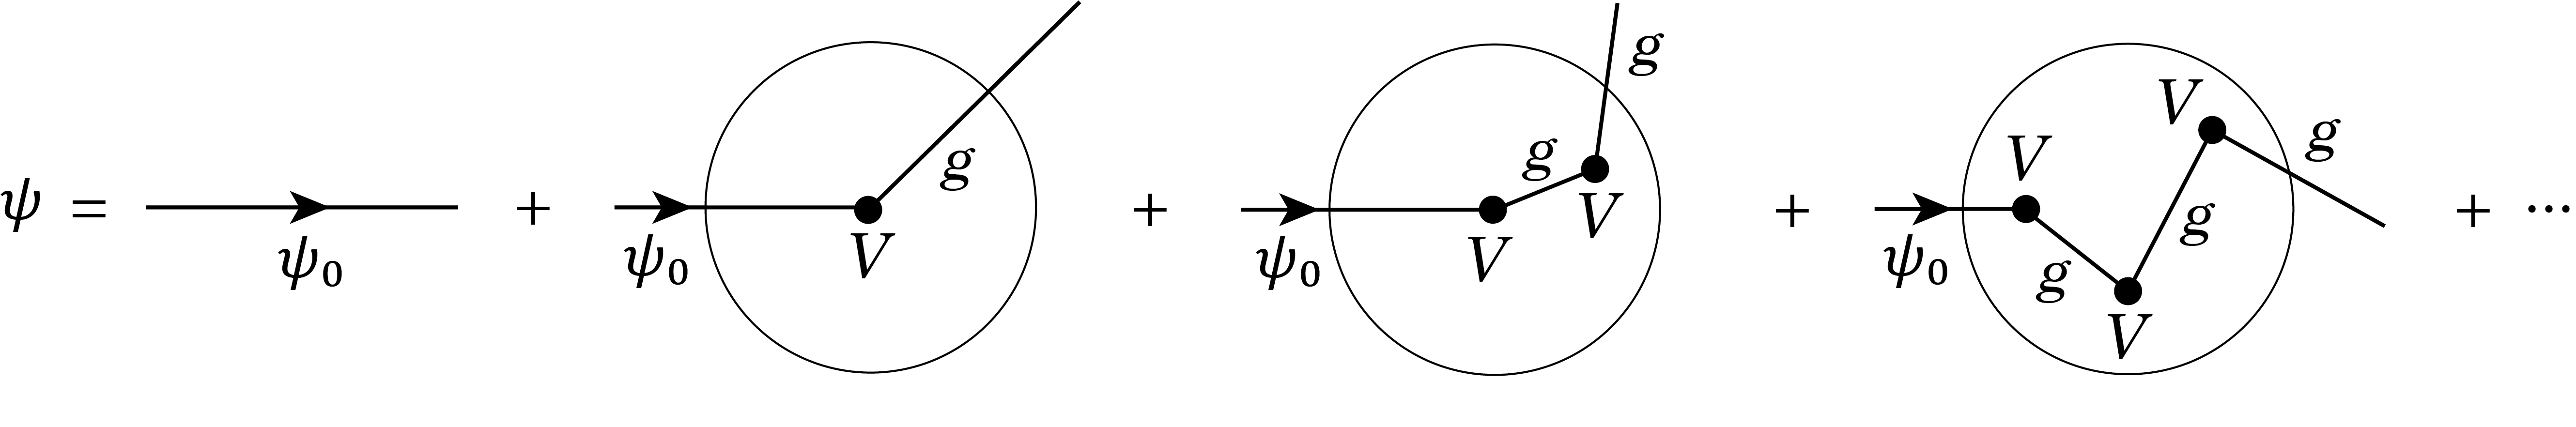
\includegraphics[width=0.9\linewidth]{class_5/images/born-diagram.png}
    \caption{Диаграмма, описывающая ряд Борна}
    \label{fig:born-series}
\end{figure}